% Rules for How Language Models Forget Facts During Training
% Build: sh build.sh   (latexmk + pdflatex, writes ../PAPER.pdf)
\documentclass{article}
\usepackage[utf8]{inputenc}
\usepackage[T1]{fontenc}
\usepackage{microtype}
\usepackage[table]{xcolor}
\usepackage{graphicx}
\usepackage{afterpage}
\usepackage{fnpos}
\makeFNabove
\usepackage{booktabs}
\usepackage{tabularx}
\usepackage{capt-of}
\usepackage{enumitem}
\usepackage{hyperref}
\newcommand{\theHalgorithm}{\arabic{algorithm}}
\usepackage[preprint]{icml2026}
\usepackage{amsmath,amssymb}
\graphicspath{{figures/}}
\renewcommand{\tabularxcolumn}[1]{>{\raggedright\arraybackslash}p{#1}}
\newcolumntype{R}[1]{>{\raggedright\arraybackslash}p{#1}}
\renewcommand{\topfraction}{0.9}\renewcommand{\bottomfraction}{0.6}\renewcommand{\textfraction}{0.07}
\renewcommand{\floatpagefraction}{0.75}\renewcommand{\dbltopfraction}{0.9}\renewcommand{\dblfloatpagefraction}{0.75}
\setcounter{topnumber}{3}\setcounter{dbltopnumber}{2}\setcounter{totalnumber}{5}
\setlist[itemize]{leftmargin=1.2em,itemsep=2pt,topsep=3pt,parsep=0pt}
\setlist[enumerate]{leftmargin=1.5em,itemsep=2pt,topsep=3pt,parsep=0pt}

\newcommand{\rowline}{\arrayrulecolor{black!25}\specialrule{0.3pt}{2.5pt}{2.5pt}\arrayrulecolor{black}}
\newsavebox{\teaserbox}

\newcommand{\kept}{\mathrm{kept}}
\newcommand{\etamax}{\eta_{\max}}
\newcommand{\he}{\hat{\eta}}
\newcommand{\hT}{\hat{T}}
\newcommand{\hw}{\hat{w}}
\newcommand{\hL}{\hat{L}}

\icmltitlerunning{Rules for How Language Models Forget Facts During Training}

\renewcommand{\today}{November 27, 2026}
\begin{document}
\twocolumn[
  \icmltitle{Rules for How Language Models Forget Facts During Training}
  \begin{icmlauthorlist}
    \icmlauthor{Vuk Rosi\'c}{ars}
  \end{icmlauthorlist}
  \icmlaffiliation{ars}{Independent researcher}
  \icmlcorrespondingauthor{Vuk Rosi\'c}{Discord: jensen404}
  \vskip 0.3in
]
\printAffiliationsAndNotice{}

% Figure 1 sits at the bottom of page 1 across both columns: the left column carries it in a
% bottom float that overflows to the right, and the right column reserves the same height.
\sbox{\teaserbox}{\begin{minipage}{\textwidth}\centering\vspace{4pt}
  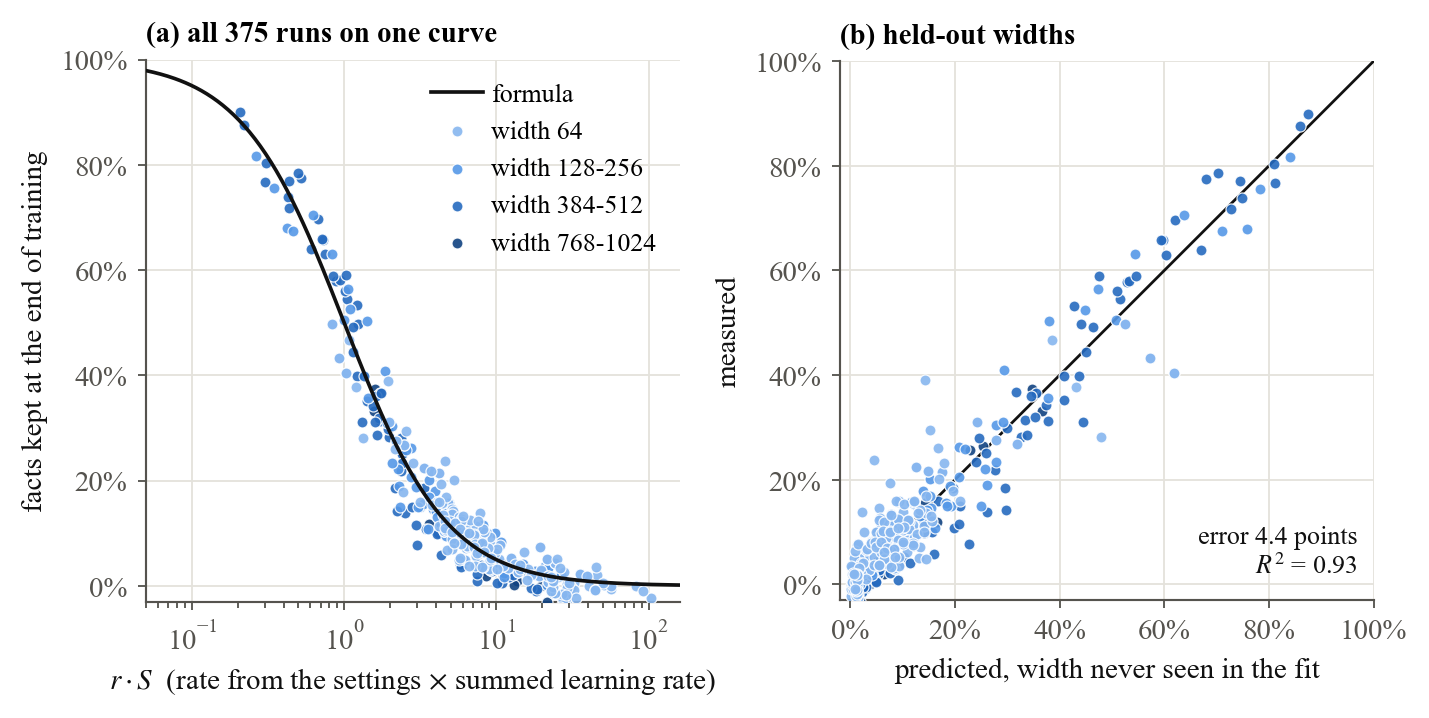
\includegraphics[width=0.8\textwidth]{fig3_one_curve}
  \captionof{figure}{One formula for all 375 runs. Each dot is one training run. (a) The share of facts kept at the end of training against $rS$: the learning rate summed after the facts ($S$) times the forgetting rate $r$ that the formula gives for the model and its settings. The line is the formula. (b) Measured against predicted, where each run is predicted by constants fitted without any run of its model width.}
  \label{fig:curve}
\end{minipage}}
\begin{figure}[b]
\makebox[\columnwidth][l]{\usebox{\teaserbox}}
\end{figure}
\afterpage{\begin{figure}[b]\rule{0pt}{\dimexpr\ht\teaserbox+\dp\teaserbox\relax}\end{figure}}

\begin{abstract}
We give seven rules for how a small language model forgets facts it stops seeing during training, each with a label for how sure we are. They come from 375 transformers (0.12M to 126M parameters) trained with Muon, with made-up facts shown in one window of each run. The main rule: facts fade with $S$, the learning rate summed over the steps after the facts, not with the number of steps. So lowering the learning rate after the facts keeps the most: a cosine schedule keeps 29\% where a constant one keeps 2\%. One formula, $\kept = 1/(1+(rS)^{q})$, turns the rules into a prediction made before training. For model widths it never saw, it is off by 4.4 percentage points, and the error does not grow with model size across a 1,000-fold range. Its one test beyond that range, a 503M-parameter model, was committed before the result: 24.1\% predicted, 24.2\% measured. The runs, formula and code are public, so the ten constants can be refitted to larger models. Repeated facts and other optimizers are not tested.
\end{abstract}

\begin{table*}[t]
\caption{Every term of the formula. The ten numbers are fitted on all 375 runs. In the second part, a term above zero makes the model forget faster and a term below zero makes it forget slower.}
\label{tab:terms}
\centering
\small
\begin{tabularx}{\textwidth}{@{}l >{\hsize=0.92\hsize}X >{\hsize=1.08\hsize}X@{}}
\toprule
\textbf{Term} & \textbf{What it is} & \textbf{What it does} \\
\midrule
\multicolumn{3}{@{}l@{}}{\textbf{Equation~\ref{eq:kept}: the share of facts kept}} \\
\addlinespace[3pt]
$\kept$ & The share of the facts the model still knows when training ends. 1 is all of them, 0 is none. & This is what the formula predicts. \\
\rowline
$S$ & The learning rate $\eta_t$ added up over every step after the facts, from step $t_0+1$ (the first step without facts) to the last step $T$. & The clock. More $S$ means fewer facts kept. The schedule fixes $S$, so it is known before training. \\
\rowline
$r$ & The forgetting rate: how fast this model, with these settings, loses facts per unit of $S$. Equation~\ref{eq:rate} gives it. & Half the facts are gone when $S$ reaches $1/r$. A larger $r$ means faster forgetting. \\
\rowline
$q = 1.282$ & The steepness of the fade. & It sets how sharply $\kept$ falls around $S = 1/r$. \\
\midrule
\multicolumn{3}{@{}l@{}}{\textbf{Equation~\ref{eq:rate}: the forgetting rate $r$, one row per term}} \\
\addlinespace[3pt]
$0.609$ & The base value. It is $\ln r$ for the reference run: width 256, 8 layers, peak 0.008, 1,024 steps, no weight decay, decay to zero. & $r = 1.84$ for the reference run. Every other term is zero there and measures a change from it. \\
\rowline
$-0.593\,\ln\he$ & Peak learning rate, $\he = \etamax/0.008$. & A higher peak lowers $r$. Doubling the peak multiplies $r$ by 0.66 at width 256. $S$ doubles at the same time, so $rS$ grows by 1.33: more forgetting, but not twice as much. \\
\rowline
$+0.848\,\lambda$ & Weight decay $\lambda$. & More weight decay, faster forgetting. A weight decay of 0.1 multiplies $r$ by 1.09, and 1.0 multiplies it by 2.33. \\
\rowline
$+0.548\,f$ & The final learning rate as a share of the peak: $f=0$ for a decay to zero, $f=1$ for a constant schedule. & A schedule that does not decay forgets faster per unit of $S$. A constant schedule multiplies $r$ by 1.73. \\
\rowline
$-1.123\,\ln\hT$ & Run length, $\hT = T/1024$ steps. & A longer run has a lower $r$. Doubling the steps multiplies $r$ by 0.46, which nearly cancels the doubled $S$. \\
\rowline
$-0.322\,\ln\hw + 0.231\,(\ln\hw)^2$ & Model width, $\hw = w/256$. & $r$ is lowest near width 512 and higher on both sides: 5.1 at width 64, 1.6 at width 512 and 1.7 at width 1,024, with the depths we ran. \\
\rowline
$+0.178\,\ln\he\,\ln\hw$ & Peak learning rate and width together. & A higher peak costs a wide model more than a narrow one. \\
\rowline
$-0.124\,\ln\hL$ & Depth, $\hL = L/8$ layers. & It adds nothing to the score (Figure~\ref{fig:parts}b). It stays because the formula was frozen with it. \\
\bottomrule
\end{tabularx}
\end{table*}

\section{Introduction}

Language models are trained in phases. Code, maths or instruction data often enters at one point of a run and does not return. By the end of training the model has lost part of what it learned from that data. A person planning such a run wants to know how much will be left, before spending the compute.

Published work measures this forgetting in steps. Chang et al. (2024) inject facts into pretraining and find that they are forgotten along a power law in the number of steps since they were last seen. A step count cannot be the whole story. A step at learning rate zero changes nothing, and a step at a high learning rate changes a lot. We use $S$, \textbf{the sum of the learning rate over every step after the facts}. It is known before training, because the schedule is known.

\textbf{The formula.} It takes settings known before training and returns the share of the facts the model still knows at the end:
\begin{equation}
\kept \;=\; \frac{1}{1+(r\,S)^{q}}, \qquad S \;=\; \sum_{t=t_0+1}^{T} \eta_t ,
\label{eq:kept}
\end{equation}
with $q = 1.282$. Here $\eta_t$ is the learning rate at step $t$, $t_0$ is the last step that shows the facts and $T$ is the last step of the run. The rate $r$ depends on the model and the settings:
\begin{equation}
\begin{aligned}
\ln r \;=\;\; & 0.609 \;-\; 0.593\,\ln\he \;+\; 0.848\,\lambda \;+\; 0.548\,f \\
 & -\; 1.123\,\ln\hT \;-\; 0.322\,\ln\hw \;+\; 0.231\,(\ln\hw)^{2} \\
 & +\; 0.178\,\ln\he\,\ln\hw \;-\; 0.124\,\ln\hL .
\end{aligned}
\label{eq:rate}
\end{equation}
Each hatted setting is divided by its value in a reference run: $\he = \etamax/0.008$ for the peak learning rate, $\hT = T/1024$ for the number of steps, $\hw = w/256$ for the model width and $\hL = L/8$ for the number of layers. $\lambda$ is the weight decay, and $f$ is the final learning rate as a share of the peak. Table~\ref{tab:terms} explains every term, and Figure~\ref{fig:curve} shows all 375 runs against the formula.

The paper is for anyone who trains a small language model in phases and wants data shown early to survive to the end. It makes three claims.

\begin{enumerate}
\item \textbf{The learning rate is the clock.} At every model size we tested, $S$ explains 93\% to 98\% of the variation in the share kept during the fade. Steps explain 48\% to 90\% (Section~\ref{sec:clock}).
\item \textbf{One formula predicts runs it never saw.} On model widths held out of the fit it is off by 4.4 percentage points of the facts, where $S$ alone is off by 15.1. Its prediction for a 503M-parameter model was committed before the result: 24.1\% predicted, 24.2\% measured (Section~\ref{sec:formula}).
\item \textbf{Seven rules follow, each with a stated certainty.} Table~\ref{tab:rules} gives the rules, Section~\ref{sec:limits} says where the formula fails, and Section~\ref{sec:todo} lists the runs that are still missing.
\end{enumerate}

The 375 runs, the formula and the scoring code are public, so every number below can be recomputed in about a minute on a laptop.


\makeFNbelow
\section{Setup}

\textbf{Models and training.} Decoder-only transformers with RMSNorm, rotary position encoding, QK-norm and SwiGLU blocks. Width runs from 64 to 1,024 and depth from 3 to 12 layers, which gives 0.12M to 126M parameters outside the embedding and output tables. Wider models are also deeper. They train on web text from FineWeb (Penedo et al., 2024) with 64 sequences of 64 tokens per step, for 512 to 4,096 steps. Muon updates the matrices inside the blocks and Adam updates the embeddings, the output table and the norms. The peak learning rate is $4\times10^{-3}$ to $32\times10^{-3}$ and the weight decay is 0 to 1.0. Most runs use a constant schedule, a cosine to zero, a cosine to 10\% of the peak, or a hold followed by a linear decay. Another 27 runs use 23 other schedule shapes.

\textbf{The facts.} We make up 64 people with five attributes each, such as birth city and employer. Short sentences such as ``Ana Reyes was born in Lisbon'' are mixed into the text during one window of the run and never return. The window covers 20\% to 45\% of the steps in 275 runs and 45\% to 70\% in 99 runs. One run shows the facts all the way through.

\textbf{What ``kept'' means.} After the window we measure the model's loss on the attribute tokens, in bits. Let $b_0$ be that loss at the end of the window, $b$ the loss later on, and $C$ the loss on facts the model barely knows. Then
\begin{equation}
\kept \;=\; 1 - \frac{b - b_0}{C - b_0}.
\end{equation}
Kept is 100\% at the end of the window and 0\% when the facts are no better known than barely seen ones. If $b_0 = 5$, $C = 35$ and $b = 20$, then kept is 50\%.

\textbf{Scoring.} A formula sees only settings chosen before training. We fit its constants on six model widths, predict the seventh, and take the root-mean-square error of kept. The score is the mean of the seven errors, in percentage points of the share kept. An error of 4.4 points means the formula says 30\% and the run keeps about 26\% or 34\%. Two numbers give the scale. Guessing the average of the other runs has an error of 21.8 points. Training the same settings twice gives results 1.3 points apart, and no formula can do better than that floor.

\section{The rules}
\label{sec:rules}

Table~\ref{tab:rules} lists the seven rules. Each has a label, and the label is defined by a test.

\begin{itemize}
\item \textbf{Strong.} The rule held on settings the fit never saw, with an error close to the 4.4 points for a new model width.
\item \textbf{Medium.} The rule holds inside the tested range, and outside it there is a known failure or too few runs.
\item \textbf{Weak.} The runs cannot separate the rule from another cause.
\end{itemize}

\begin{table*}[t]
\caption{The rules, the evidence for each, and how sure we are.}
\label{tab:rules}
\centering
\small
\begin{tabularx}{\textwidth}{@{}c R{0.23\textwidth} X R{0.25\textwidth}@{}}
\toprule
\textbf{\#} & \textbf{Rule} & \textbf{Evidence} & \textbf{How sure} \\
\midrule
1 & Facts fade with the learning rate summed after them ($S$), not with the number of steps. & $S$ explains 93\% to 98\% of the fade at all ten model sizes, steps 48\% to 90\%. For a schedule shape the fit never saw, the error is 2.8 points with $S$ and 7.2 with steps. & \textbf{Strong} \\
\rowline
2 & One formula gives the share kept at the end of training. & Error of 4.4 points for a new width, 2.8 for a new schedule, 4.1 for a new peak, 4.3 for a new depth, 5.1 for a new run length. One prediction committed first: 24.1\% against 24.2\%. & \textbf{Strong} at the end of training. \textbf{Medium} inside the run (8.0 points) \\
\rowline
3 & Lowering the learning rate after the facts keeps the most. A learning rate that never decays costs extra. & Same steps and peak: a constant schedule keeps 2\%, a cosine keeps 29\%. A constant schedule also multiplies $r$ by 1.73. & \textbf{Strong} \\
\rowline
4 & A higher peak costs less than its size, least in small models. & Doubling the peak multiplies $rS$ by 1.12 at width 64, 1.33 at width 256 and 1.57 at width 1,024. Error of 4.1 points for a new peak. & \textbf{Medium}: widths 768 and 1,024 have 6 runs each \\
\rowline
5 & Weight decay speeds forgetting. & Runs that differ only in weight decay keep less with it: in 34 of 48 pairs at 0.1, 37 of 38 at 0.3 and 24 of 24 at 1.0. & \textbf{Medium}: fitted without the runs at weight decay 0, the formula misses them by 33.8 points \\
\rowline
6 & Facts shown later are kept more. & In 83 pairs of runs that differ only in the fact window, the early window keeps 10.7\% on average and the late one 35.6\%. The late one keeps more in all 83. & \textbf{Medium}: the direction is certain, the amount is not (8.5 points across windows, two windows only) \\
\rowline
7 & A longer run forgets about the same share. & Doubling the steps multiplies $rS$ by 0.92. Error of 5.1 points for a new run length. & \textbf{Weak}: the fact window grows with the run, so the two cannot be separated \\
\bottomrule
\end{tabularx}
\end{table*}

All seven rules are for facts shown in one window and never again. No run shows the facts a second time, so the rules say nothing about repeated facts. Width and depth are not in the table: in our runs deeper models are also wider, so we cannot say which of the two changes forgetting. Appendix~\ref{app:rules} explains rules 3 to 7 one by one.

\section{The learning rate is the clock}
\label{sec:clock}

Figure~\ref{fig:idea} shows the effect on one model. Four runs at width 512 share everything except the schedule, so all four have the same 564 steps after the facts. A step count predicts the same loss for all four. They end with 2.0\%, 9.9\%, 28.0\% and 28.6\% of the facts. Their $S$ values are 4.51, 2.46, 1.36 and 1.00, in the same order.

\begin{figure*}[t]
\centering
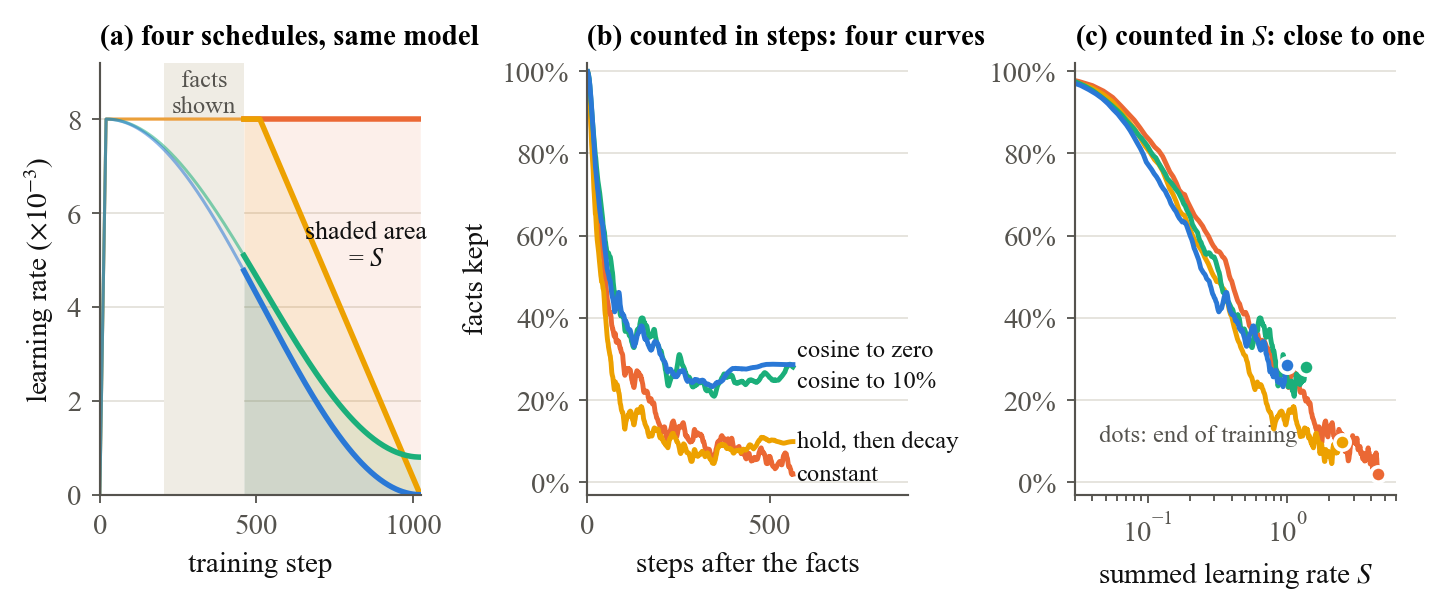
\includegraphics[width=0.92\textwidth]{fig1_idea}
\caption{The idea, on four runs of the same 21M-parameter model that differ only in the learning-rate schedule. (a) The facts are shown during the grey window. $S$ is the area under the learning-rate curve after the window. (b) Counted in steps, the four runs lose the facts along four different curves. (c) Counted in $S$, they follow nearly one curve. The formula is that one curve, with a rate that depends on the model and the settings.}
\label{fig:idea}
\end{figure*}

To test this at every model size, we take every reading inside the fade from all runs of one size with 1,024 steps and no weight decay. We fit the same three-constant curve twice, once with the number of steps as the clock $c$ and once with $S$:
\begin{equation}
\kept \;=\; \frac{1}{1+\bigl(a\,\etamax^{\,g}\,c\bigr)^{q}} .
\end{equation}
Both versions get their own $a$, $g$ and $q$ for each model size. The exponent $g$ lets steps use the peak learning rate too, so the comparison is fair to steps.

\begin{figure}[t]
\centering
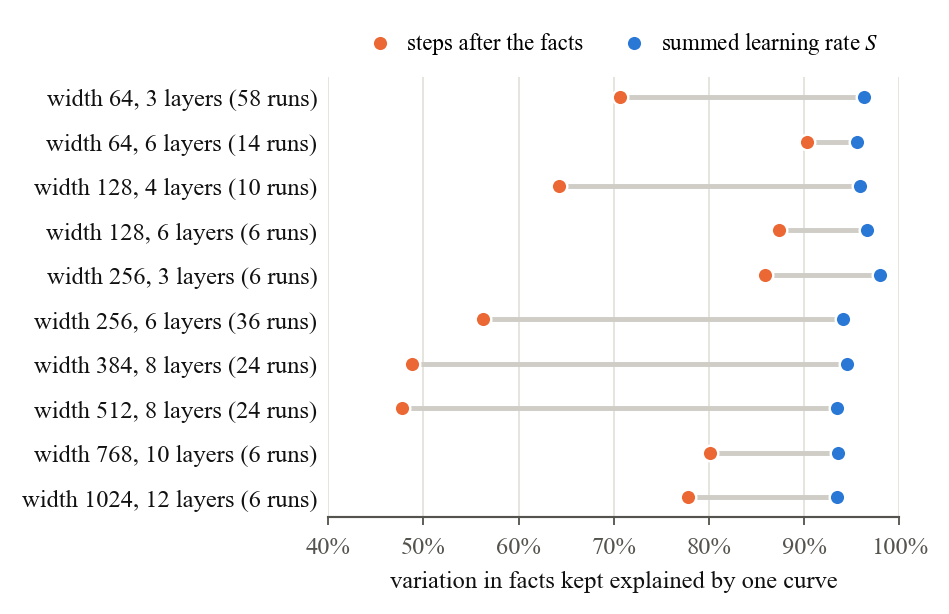
\includegraphics[width=\columnwidth]{fig2_clock}
\caption{$S$ explains the fade better than steps at every model size. Each row is one model size. The dots show how much of the variation in kept one curve explains when the clock is the number of steps since the facts (orange) or the summed learning rate $S$ (blue). Both curves have three constants.}
\label{fig:clock}
\end{figure}

$S$ wins at all ten model sizes (Figure~\ref{fig:clock}). It explains 93\% to 98\% of the variation, and steps explain 48\% to 90\%. The gap is largest where a model size has runs with several schedules, because that is where steps and $S$ disagree: at width 512, 48\% against 93\%.

Why would $S$ be the clock? This is a guess that we did not test. Muon makes each update of a weight matrix the same size in every direction, scaled by the learning rate. The total distance the weights can move after the facts is then close to $S$. A fact is stored in the weights, and it is lost as later updates move them.

\section{One formula predicts runs it never saw}
\label{sec:formula}

Equations~\ref{eq:kept} and~\ref{eq:rate} give the formula and Table~\ref{tab:terms} explains its terms. The rate $r$ says how fast a model with given settings loses facts per unit of $S$, and half the facts are gone when $S$ reaches $1/r$. An example: a 21M-parameter model (width 512, 8 layers) trains for 1,024 steps at peak $8\times10^{-3}$ with a cosine to zero. Then $S = 1.00$ and $r = 1.64$, so the formula says 34\% kept. The run kept 29\%. With a constant schedule $S = 4.51$ and $r = 2.84$, the formula says 4\%, and the run kept 2\%.

Figure~\ref{fig:curve}a puts all 375 runs on one axis, $rS$. They fall on one curve. The error of this fit is 3.8 points.

A fit can look good because it has seen the data. Figure~\ref{fig:curve}b shows the test that counts. Each point is predicted by constants fitted without any run of that width. The error is 4.4 points, and the predictions explain 93\% of the variation in kept. Half of the runs are predicted within 2.7 points and 95\% within 10 points. On the 176 runs that keep at least 10\% of the facts, where a constant guess near zero cannot help, the error is 6.6 points.

Three simpler predictors do worse under the same test. The average of the other widths is off by 21.8 points. $S$ alone, with two constants and no settings, is off by 15.1. The full formula with the number of steps in place of $S$ is off by 8.0. Appendix~\ref{app:terms} removes the terms one at a time.

The error does not grow with model size. At the seven held-out widths it lies between 3.1 and 6.2 points, with 5.1 at width 64 and 3.1 at width 1,024.

\textbf{A prediction committed before the result.} Held-out scores can still flatter a formula, because the person who writes it has seen the whole table. A prediction for a run that does not exist yet cannot be tuned. We wrote down what the formula predicts for a model of width 2,048 with 12 layers. It has 503M parameters, four times more than the largest model in the table. The prediction was committed to the public repository at 00:35 on 27 November 2026 (commit \texttt{19e61cc}), and the result at 02:09 (commit \texttt{da0449e}). The formula predicted 24.1\% kept and the run kept 24.2\%.

The prediction was not a copy of the nearest runs. With this schedule and peak, the table has 31\%, 32\% and 29\% at widths 256, 384 and 512, which carried forward gives about 30\%. The squared width term bends the rate back up, so the formula said 24\%.

This is one run. A miss of 0.02 points is far below the floor of 1.3 points, so part of the match is luck. Appendix~\ref{app:prediction} gives the details and three earlier checks where the formula was too high.

\begin{table*}[t]
\caption{Future work: the open questions and the runs that would answer them. The first three rows come first.}
\label{tab:todo}
\centering
\small
\begin{tabularx}{\textwidth}{@{}R{0.15\textwidth} X X@{}}
\toprule
\textbf{Open question} & \textbf{Runs that would answer it} & \textbf{What it would change} \\
\midrule
Repeated facts & Show the same facts in two or three windows, with gaps of 10\% to 40\% of the run, at widths 64 and 256 and four schedules. & Whether $S$ counts from the last showing, and whether a second showing lowers $r$. The formula has no term for this. \\
\rowline
The cause & Measure how far the weights move after the facts under each schedule and compare it with $S$. & Turns the guess at the end of Section~\ref{sec:clock} into a tested cause. \\
\rowline
Other optimizers & The same runs at widths 64 and 256 with Adam on all weights, and with SGD with momentum. & Whether $S$ is the clock outside Muon (rule 1). \\
\rowline
Facts at other times & Windows at 5\% to 30\% and 70\% to 95\% of the run, and windows of different length at a fixed run length. & A term for when the facts were written (rule 6). It also separates run length from window length (rule 7). \\
\rowline
Small weight decay & Weight decay 0.01 and 0.03, and runs with and without weight decay at widths 768 and 1,024. & The shape of the weight decay term near zero, where the linear term fails (rule 5). \\
\rowline
Width against depth & Widths 512 to 1,024 with 3 or 4 layers, and widths 64 to 128 with 10 or 12 layers. & Which of the width and depth terms is real. Wide, shallow models are overpredicted today. \\
\rowline
More predictions made first & Several models above 500M parameters and runs of 100,000 steps or more, each with a committed prediction. & Rule 2 rests on one such run. This shows whether the constants hold at scale. \\
\rowline
Batch size & 16, 32, 128 and 256 sequences per step. & A batch-size term. The one bad miss we know of used 96. \\
\rowline
Real facts & Facts written in varied wording and mixed with related text. & Whether template facts fade like real knowledge. \\
\bottomrule
\end{tabularx}
\end{table*}

\section{Where the formula breaks}
\label{sec:limits}

Figure~\ref{fig:holdouts} holds out each setting in turn: fit on the other values and predict the missing one.

\begin{figure}[t]
\centering
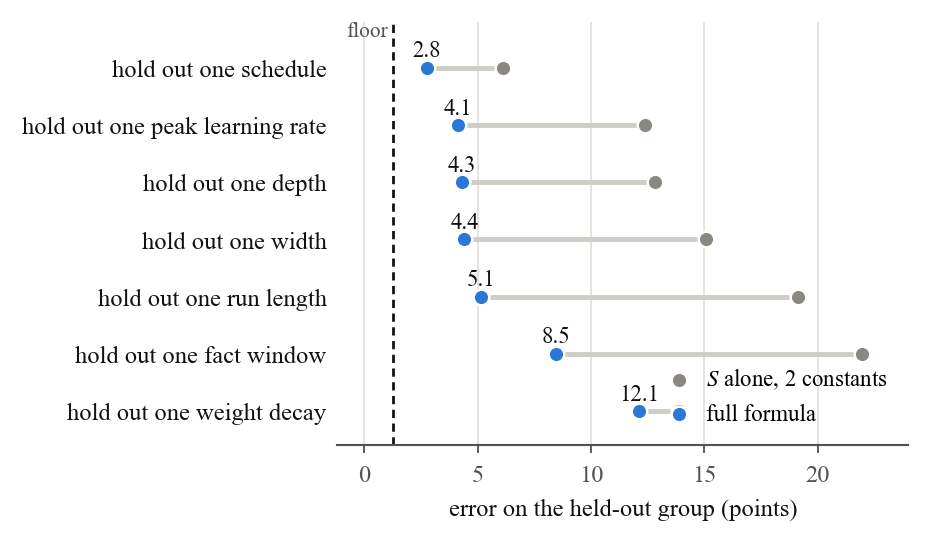
\includegraphics[width=\columnwidth]{fig4_holdouts}
\caption{Hold out each setting in turn. Each row fits the formula without one value of a setting (one schedule, one peak learning rate, and so on) and predicts the runs that have it. Numbers are the error of the full formula in percentage points. Grey dots are $S$ alone.}
\label{fig:holdouts}
\end{figure}

A new schedule shape, peak learning rate, depth or run length is predicted about as well as a new width: 2.8, 4.1, 4.3 and 5.1 points. The formula fails or is untested in these cases.

\begin{itemize}
\item \textbf{The time of the facts.} Fitted on one fact window, the formula predicts the other with an error of 8.5 points. It has no term for when the facts were shown.
\item \textbf{Weight decay far from the fitted values.} With weight decay 0.1, 0.3 or 1.0 held out, the error is 2.2, 6.1 and 6.3 points. With weight decay 0 held out it is 33.8 points.
\item \textbf{Readings inside the run.} The constants were fitted on the end of each run. Inside the fade the error is 8.0 points, and the formula is too high early on.
\item \textbf{Wide and shallow models.} Three runs at widths 512 to 1,024 with 3 layers were predicted 2 to 5 points too high.
\item \textbf{Batch size.} Every fitted run uses 64 sequences per step. One run with 96 kept 10.4\% where the formula says 28.9\%.
\item \textbf{Scale.} One prediction above 126M parameters. The longest run has 4,096 steps and 17M tokens. Of the 375 runs, 227 are 64 wide and only 6 each are 768 and 1,024 wide.
\item \textbf{Everything else we held fixed.} One optimizer, made-up facts in template sentences, and facts shown once.
\item \textbf{The floor.} The floor of 1.3 points was measured on repeated runs in our run log and cannot be recomputed from the public table. In that table 25 rows repeat another row. Without them the error is 4.3 points instead of 4.4.
\end{itemize}

\section{What needs to be done}
\label{sec:todo}

Table~\ref{tab:todo} lists the runs this paper leaves as future work. Three come first. Repeated facts, because real training data shows a fact more than once. A measurement of how far the weights move after the facts, which would test the cause we guess in Section~\ref{sec:clock}. And a second optimizer, which shows whether $S$ is the clock outside Muon. All three can be run at widths 64 to 256. The data and code are public, so each row can be run and the ten constants refitted without us.

\section{Related work}

Chang et al. (2024) inject facts into pretraining and report a power law in the number of steps since the last exposure. With one fixed schedule, steps and $S$ are the same thing up to a factor, and they differ as soon as schedules differ. Bordt et al. (2025) relate the forgetting of benchmark examples to weight decay, and Liao et al. (2024) propose entity-level measures of forgetting. None gives a formula over training settings.

Tissue et al. (2024) and Luo et al. (2025) predict the pretraining loss from the area under the learning-rate curve. Wang et al. (2025) apply the same area to the loss on an old domain during continual pretraining, which is the closest work. We use the same clock for the share of specific facts kept after a short window inside one run, under Muon (Jordan et al., 2024), with a rate fitted across model sizes and a prediction committed before its test. Kalajdzievski (2024) fits a power law for forgetting during fine-tuning.

\section{Conclusion}

A small transformer trained with Muon forgets facts it has stopped seeing according to the learning rate summed after them, not the number of steps. One formula built on this predicts the share kept at the end from the training settings. It is off by 4.4 points on model widths it never saw, the error does not grow with model size, and it predicted one 503M-parameter run before the result existed. The practical rule: to keep what a model learned early, lower the learning rate after it. The first missing test is facts that are shown more than once.

\section*{References}
{\raggedright
\begin{list}{}{\setlength{\leftmargin}{1em}\setlength{\itemindent}{-1em}\setlength{\itemsep}{3pt}\setlength{\parsep}{0pt}\setlength{\topsep}{2pt}}
\item Bordt, S., Srinivas, S., Boreiko, V., and von Luxburg, U. (2025). How much can we forget about data contamination? In \textit{International Conference on Machine Learning (ICML)}. arXiv:2410.03249.
\item Chang, H., Park, J., Ye, S., Yang, S., Seo, Y., Chang, D.-S., and Seo, M. (2024). How do large language models acquire factual knowledge during pretraining? In \textit{Advances in Neural Information Processing Systems (NeurIPS)}. arXiv:2406.11813.
\item Jordan, K., Jin, Y., Boza, V., You, J., Cesista, F., Newhouse, L., and Bernstein, J. (2024). Muon: an optimizer for hidden layers in neural networks. \url{https://kellerjordan.github.io/posts/muon/}.
\item Kalajdzievski, D. (2024). Scaling laws for forgetting when fine-tuning large language models. arXiv:2401.05605.
\item Liao, C., Xie, R., Sun, X., Sun, H., and Kang, Z. (2024). Exploring forgetting in large language model pre-training. arXiv:2410.17018.
\item Luo, K., Wen, H., Hu, S., Sun, Z., Liu, Z., Sun, M., Lyu, K., and Chen, W. (2025). A multi-power law for loss curve prediction across learning rate schedules. arXiv:2503.12811.
\item Penedo, G., Kydl\'i\v{c}ek, H., Ben allal, L., Lozhkov, A., Mitchell, M., Raffel, C., Von Werra, L., and Wolf, T. (2024). The FineWeb datasets: decanting the web for the finest text data at scale. arXiv:2406.17557.
\item Tissue, H., Wang, V., and Wang, L. (2024). Scaling law with learning rate annealing. arXiv:2408.11029.
\item Wang, X., Tissue, H., Wang, L., Li, L., and Zeng, D. D. (2025). Learning dynamics in continual pre-training for large language models. In \textit{International Conference on Machine Learning (ICML)}. arXiv:2505.07796.
\end{list}}

\newpage
\appendix
\onecolumn
\raggedbottom

\section{What each term buys}
\label{app:terms}

Figure~\ref{fig:parts}a compares the formula with simpler predictors under the same test. The average of the other widths is off by 21.8 points. $S$ alone, with two constants and no settings, is off by 15.1. The full formula is off by 4.4, which is 3.5 times the floor of 1.3 points. The same formula with the number of steps in place of $S$ is off by 8.0 (Section~\ref{sec:clock}).

\begin{figure}[h]
\centering
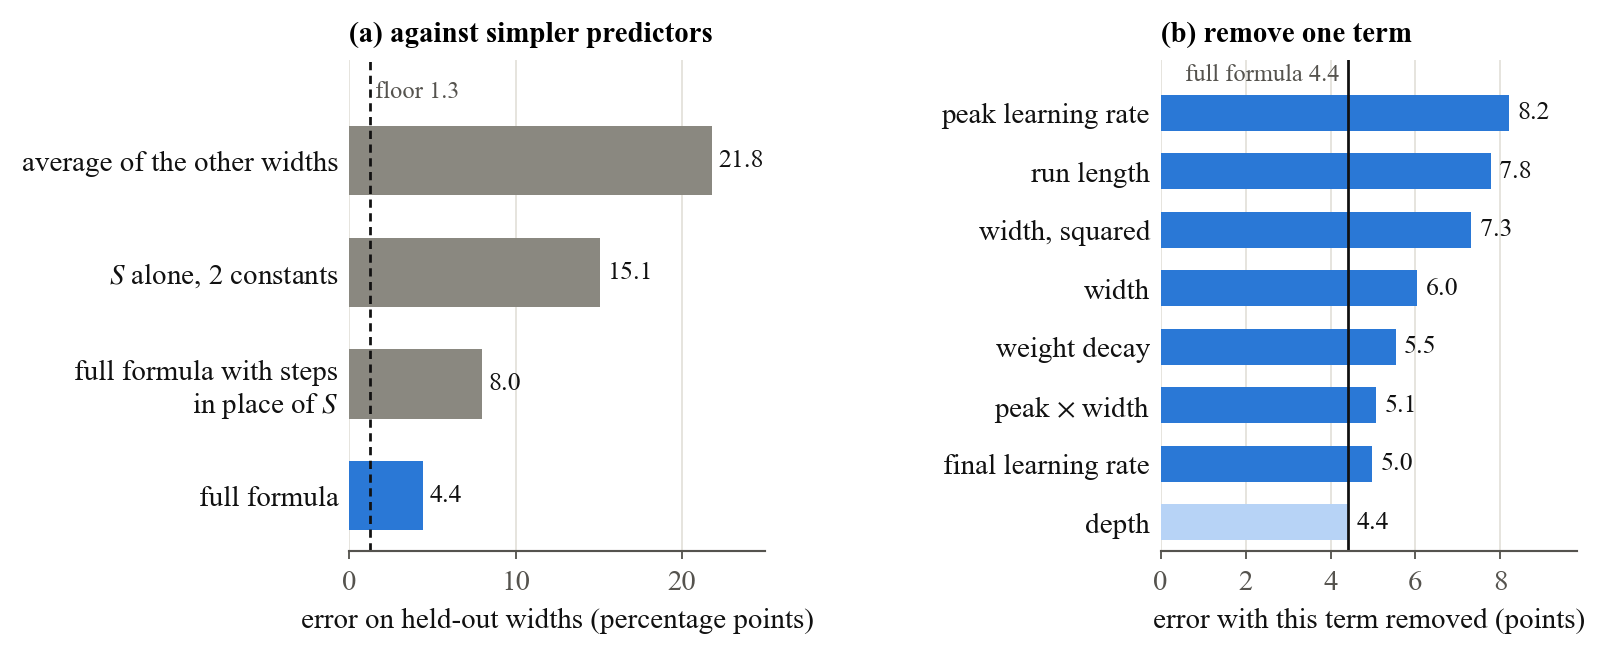
\includegraphics[width=0.74\textwidth]{fig5_parts}
\caption{What each part of the formula buys. (a) Error on held-out widths for four predictors, in percentage points of the facts kept. The dashed line is the floor, the noise between two measurements of the same settings. (b) Error when one term is removed and the rest refitted. Removing the depth term changes nothing.}
\label{fig:parts}
\end{figure}

Figure~\ref{fig:parts}b removes one term at a time and refits. The peak learning rate, the run length and the width terms matter most: without any one of them the error is 6.0 to 8.2 points. The depth term does not matter. Without it the error is still 4.4 points. Width and depth grow together in this table, so the width terms already carry what depth would add. We keep the depth term because the formula was frozen and its prediction committed with it (Section~\ref{sec:formula}), but a nine-constant version does the same job.

\section{Rules 3 to 7 in detail}
\label{app:rules}

\textbf{Rule 3. Lower the learning rate after the facts.} $S$ is the area under the schedule after the facts. Moving area from after the facts to before them is the cheapest way to keep more. In Figure~\ref{fig:idea}, replacing a constant schedule by a cosine cuts $S$ from 4.51 to 1.00 and raises kept from 2\% to 29\%, with the same steps and the same peak. A constant schedule costs twice: it has the largest $S$, and it multiplies $r$ by 1.73. The last steps of a decaying schedule do almost no damage, and some facts recover slightly while the learning rate falls (Figure~\ref{fig:idea}b, cosine to zero).

\textbf{Rule 4. A higher peak costs less than its size.} Doubling the peak doubles $S$, but $r$ falls. The product $rS$ grows as the peak to the power 0.16 at width 64, 0.41 at width 256 and 0.65 at width 1,024. A small model forgets almost the same share at any peak. A wide model is more sensitive. The label is medium because the two widest models have 6 runs each.

\textbf{Rule 5. Weight decay speeds forgetting.} In the formula, weight decay 0.1 multiplies $r$ by 1.09, 0.3 by 1.29 and 1.0 by 2.33. The runs agree. Pairs of runs that differ only in weight decay keep 10.5\% without it and 8.0\% with 0.1, 22.1\% and 16.0\% with 0.3, and 15.7\% and 8.0\% with 1.0. The label is medium because the term does not extrapolate: fitted only on runs with weight decay, the formula misses the runs without it by 33.8 points (Section~\ref{sec:limits}).

\textbf{Rule 6. Facts shown later are kept more.} We ran 83 settings with both fact windows. Facts shown at 20\% to 45\% of the run end at 10.7\% kept on average. Facts shown at 45\% to 70\% end at 35.6\%, and they are higher in all 83 pairs. Part of this is rule 1: fewer steps remain after a later window, so $S$ is smaller. The formula has no other term for the time of the facts, and across windows its error is 8.5 points. So the direction is certain and the amount is not.

\textbf{Rule 7. A longer run forgets about the same share.} Doubling the number of steps with the same schedule shape doubles $S$ and multiplies $r$ by 0.46, so $rS$ changes by a factor of 0.92. The fact window is a fixed share of the run here, so a longer run also has a longer window and the model sees each fact more often. The table cannot separate the two effects, which is why the label is weak.

\section{The committed prediction in detail}
\label{app:prediction}

We fitted three formulas on the 375 runs: the one in this paper and two longer ones with 12 and 13 constants. Both add a batch-size term and an extra term for wide models with early facts. The longest also lets the steepness $q$ change with width. We wrote down what each predicts for a model of width 2,048 with 12 layers. It has 503M parameters, four times more than the largest model in the table. The predictions were committed to the public repository at 00:35 on 27 November 2026 (commit \texttt{19e61cc}). The result was committed at 02:09 (commit \texttt{da0449e}).

The run kept 24.2\% of the facts (0.2416). The formula of this paper predicted 24.1\% (0.2414). The two longer formulas predicted 22.3\% and 18.9\% (Figure~\ref{fig:prediction}b).

\begin{figure}[h]
\centering
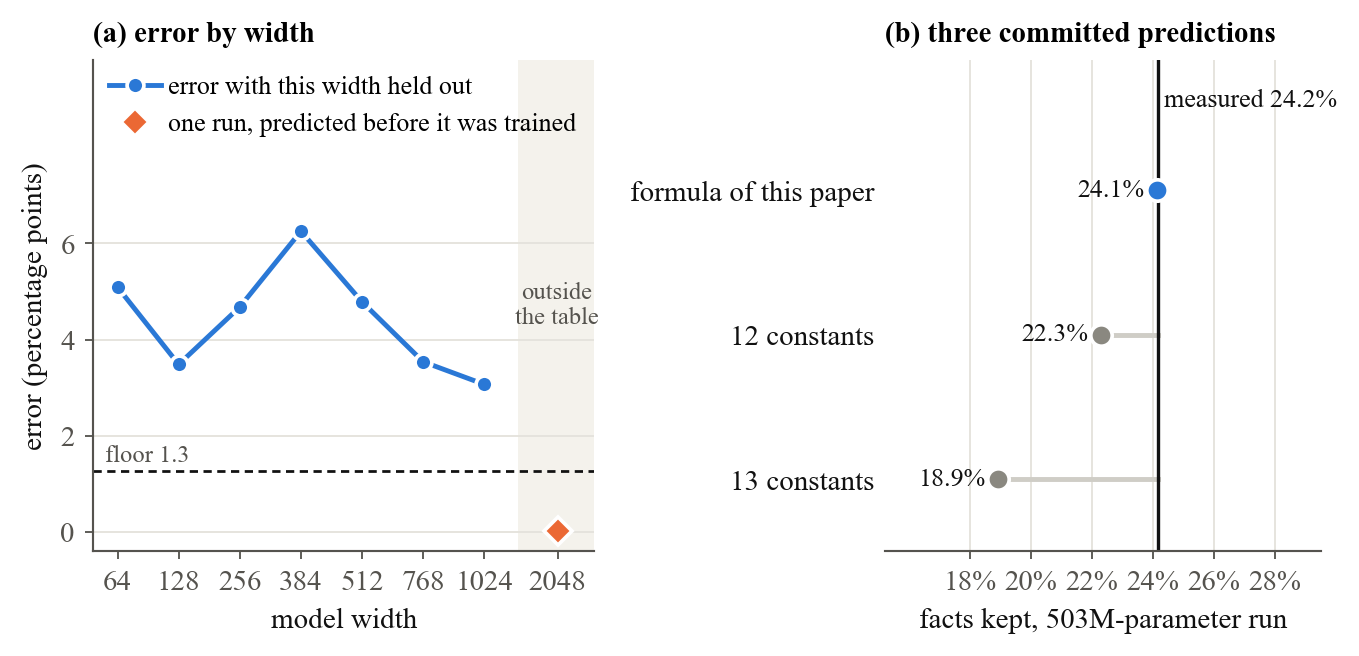
\includegraphics[width=0.68\textwidth]{fig6_prediction}
\caption{The committed prediction. (a) Error by model width. Blue: the error on each width when it is held out of the fit. Orange: the 503M-parameter run, predicted before its result existed and four times larger than any model in the table. (b) What the three committed formulas predicted for that run. The vertical line is the measured value.}
\label{fig:prediction}
\end{figure}

The prediction was not a copy of the nearest runs. With this schedule and peak, the table has 12\% kept at width 64 and 31\%, 32\% and 29\% at widths 256, 384 and 512. Carrying the last values forward gives about 30\% at width 2,048. The squared width term bends the rate back up, so the formula predicted 24\%, less than at width 512. The result agreed.

This is one run, and we do not claim more for it than that. A miss of 0.02 percentage points is far below the floor of 1.3 points, so part of the match is luck. The run used 32 sequences per step and every run in the table used 64. The formula has no batch-size term, and the two formulas that have one predicted lower. A second run at half the peak, with a committed prediction of 38.8\%, was withdrawn and has no result.

Two earlier checks point the other way. Three runs at widths 512 to 1,024 with only 3 layers were predicted before they finished, in our notebook and not in git. The formula was too high on all three, by 2 to 5 points. One run finished before the predictions were committed and so proves nothing about order, but it shows the size of a bad miss: width 768, weight decay 0.3, 96 sequences per step and 2,048 steps. It kept 10.4\% of the facts and the formula says 28.9\%.

\section{Reproduce}

The data, the formula and the scoring code are in \texttt{github.com/vukrosic/training-law-finder}.

{\small
\begin{verbatim}
git clone https://github.com/vukrosic/training-law-finder
cd training-law-finder
# score on held-out widths: prints 0.0441, which is 4.4 points
python3 core/score.py forgetting problems/forgetting/formulas/end_z2.py --family llm
# the committed prediction and the known miss
python3 core/round_score.py rounds/002-forgetting
# every number and figure of this paper, from the two scripts next to it (no training)
export TLF_REPO=/path/to/training-law-finder
python3 paper_numbers.py   # writes numbers.json
python3 make_figs.py       # writes figs/
\end{verbatim}
}

\end{document}
